\documentclass[12pt]{article}
\usepackage{amsmath}
\usepackage[margin=.9in]{geometry}
\usepackage{enumitem}
\usepackage{float}
\usepackage{graphicx} % Required for inserting images
\usepackage{helvet}
\usepackage{hyperref}
\usepackage{listings}
\usepackage{mathptmx}
\usepackage{nameref}
\usepackage{pgfplots}
\usepackage{wrapfig}
\renewcommand{\familydefault}{\sfdefault}


\title{Complex Systems and Networks HW 1}
\author{Rachael Judy, Connor Klein, Josh Smith}

\begin{document}
\pgfplotsset{compat=1.18}
\setlist[itemize]{noitemsep}
\setlist[enumerate]{noitemsep}
 
\maketitle

\section{Q1: Annotated Bibliography}
% The general topic is research on stock market analysis, important features in a complex network for the stock market, and previous techniques
% key things we're going to need:
%	- we must select our own key features for our brokers
%   - we need to decide which aspects of the complex system we're able to change/gather intel from
%   - we need to select stocks representative of various aspects of the market

Economic markets are extremely volatile and dynamic and present an active area of research. Previous models of the market treat it as a linear system, which does not fully capture the actual behavior of the market. Developing an accurate model of the market would result not only in a significant economic advantage but provide the possibility of analyzing global financial systems, market sentiment, inter-dependencies, and macroeconomic indicators. Due to the readily available detailed historical data of the stock market and the aforementioned advantages gained by correctly modeling the market, this field has been studied by numerous research groups. Within this general field, specific areas of research have included correctly modeling the markets as complex networks, forecasting stock prices in various global markets based on feature selection and through various means, examining the impact of risk and risk aversion in returns and portfolios, detecting anomalies in the market, and studying information diffusion in the market. Each of these features represents a parameter that can be adjusted in modeling the market. By reviewing previous and active research in the field of analyzing the stock market with networks, new parameters and methods for network models can be developed.

Modeling the stock market as a complex network involves viewing entities, stocks, or market groups as interconnected nodes with edges representing their relationships, whether these are transactions performed or correlations. The various parameters of the brokers and stocks can be adjusted to try to emulate the real world. This approach provides new perspectives on market dynamics, allowing analysts to discover previously unknown relationships and dependencies not apparent in traditional methods that fail to capture the influence of nodes on one another. This provides key advantages of capturing emerging trends and recognizing feedback loops. Leveraging tools such as power law, q-theory, centrality measures, and neural networks, researchers can identify critical entities and groups and better understand the forces at play.

The papers summarized here discuss the general modeling approaches taken for representing financial markets and impacts of shock events in those markets in terms of complex systems. This includes examining examining broker and stock networks from above and highlighting means for determining clusters, node parameters, and edges in the graphs through correlation, mutual information, risk, and information diffusion. Further, they discuss the results of several models in different global markets.


\subsection{Explaining financial markets in terms of complex systems}
M. Kuhlmann, "Explaining financial markets in terms of complex systems," \textit{Philosphy of Science}, vol. 81, no. 5, pp. 1117-1130, Dec. 2014. %doi: 10.1086/677699.
\newline

This paper theorizes that the US financial market can be modeled as a nonlinear complex system, based on econophysics, which explains economic phenomena with methods and models used to describe physical phenomena. Kuhlmann compares the market to a ferromagnet, in which microprocesses accumulate to create macro effects. These microprocesses are not random and linear but stem from the state of their neighbors. From this model, some of the microprocesses can be filtered out, resulting in the larger macro functions being derived without full information. He postulates that the structural mechanisms can be broken into two classes: a structural start with boundary conditions and emerging dynamical systems from those conditions. This can be seen as a similar underlying structure with an entirely different function. This paper describes how the financial market could be modeled as a complex network, but does not discuss specific modeling parameters; instead, Kuhlmann highlights the failure of current models due to unrealistic modeling of human behavior which do not address the structural mechanisms of interacting agents. Thus, the work is primarily a thought experiment requiring further work to advance the modeling of the complexity of human interactions through these structural networks.


\subsection{The relevance of broker networks for information diffusion in the stock market}
M. Di Maggio, F. Franzoni, A. Kermani, and C. Sommavilla, "The relevance of broker networks for information diffusion in the stock market," \textit{Journal of Financial Economics}, vol. 134, no. 2, pp. 419-446, Nov. 2019. %doi: 10.1016/j.jfineco.2019.04.002. 
\newline

This report was compiled by the Harvard Business School to examine the effect of the centrality of brokers in the US stock market. The research theorizes that brokers play a key role in diffusing information from originators to investors. They examine features creating broker connections such as brokers seeking clients, clients seeking expertise, and the broker's centrality and information availability. They analyze data from 1999 to 2014 on trades and connections. They found that traders were more likely to follow large trades made by hedge fund investors with the same broker, but also central brokers — those with the most connections — had clients who, on average, performed 40 points better than peripheral brokers. They also checked that the quality of clients was not the separating factor among the brokers. The researchers concluded that connections were more significant than skill in the US financial market. They then developed an equation to estimate the performance of an active investor based on their broker’s centrality and relationship with that broker. This research was thorough in data variety and studying factors to examine the importance of brokers. Further work should include modeling the market as a set of centralized and peripheral brokers for market prediction.


\subsection{Contagion in financial networks}
P. Gai and S. Kapadia, "Contagion in financial networks," \textit{Proceedings of the Royal Society}, vol. 466, no. 2120, pp. 2401–2423, Aug. 2010.
\newline

This paper presents a model of contagion for unexpected shocks in arbitrary network structures in finance and uses numerical simulations with edges initialized by a Poisson random graph to illustrate the results. They authors discuss both the benefit of being able to absorb loss of one institution among other entities, reducing the probability of failure, and the danger of more linkages increasing the potential for spread and damage from the second round of defaults. Their directed network of interconnected balance sheets examines the number of vulnerable nth neighbors for each entity and uses recursive equations to consider possible contagion and identify phase transitions representing thresholds for outbreaks. The paper also briefly addressed how illiquid assets that are sold on default can be reduce prices generally in the liquid market, introducing a second potential source of contagion upon default. Their model has the advantage of representing arbitrary network structures not dependent on the real world model. However, the paper focused on a single disruptive event, namely the default of a single bank, and other events cannot be assumed to have the same effects. Additionally, the analytical method treated the network of a failing bank as a tree with no cycles, reducing the value of the numerical simulation results.




\subsection{A network perspective of the stock market}
C. K. Tse, J. Liu, and F. C. M. Lau, “A network perspective of the stock market,” \textit{Journal of Empirical Finance}, vol. 17, no. 4, pp. 659–667, Sep. 2010. % doi: 10.1016/j.jempfin.2010.04.008.
\newline

% review
This paper presents network constructions of US stocks and proposes a new methodology for computing stock indices. The nodes of the networks consist of stocks, and the edges are established with a winner-take-all approach based on a threshold for cross correlation of daily stock prices, price returns, and trading volumes. The networks display a power-law distribution and suggest that the majority of stocks' time indices are strongly influenced by a small subset of stocks, particularly in the financial sector. They propose a new approach of using the networks for selection of stocks to represent the market indices. The paper highlights some flaws that may be present in the current methodology of determining stock indices and expands the importance of interconnectivity in examining the stock market. However, their methods are not examined over enough data to generalize the approach; the two windows examined by the authors are each two years in length and centered around the financial crisis of 2007-2008 which may not represent the overall market over time. Further, it does not examine the impact of adjusting several somewhat arbitrary parameters such as the threshold for creating an edge.


\subsection{Pearson correlation coefficient-based performance enhancement of broad learning system for stock price prediction}
G. Li, A. Zhang, Q. Zhang, D. Wu, and C. Zhan, “Pearson correlation coefficient-based performance enhancement of broad learning system for stock price prediction,” \textit{IEEE Transactions on Circuits and Systems II: Express Briefs}, vol. 69, no. 5, pp. 2413–2417, May 2022. %, doi: 10.1109/TCSII.2022.3160266.
\newline

In this paper, the Pearson Correlation Coefficient (PCC), a measure of strength and direction of the relationship between two variables, is used with a Broad Learning System (BLS) for feature selection to perform time series prediction of stocks selected from the Shanghai Stock Exchange. The authors compare the results of their method with ten machine learning methods including Adaboost, Gradient Boosting Decision Tree, Convolutional Neural Networks, and others. The BLS system is based on a random vector functional link neural network that transforms input features to feature nodes that connect to the output layer. Weights are initially randomly generated and then improved through pseudoinversion. This provides a less time intensive alternative to a deep learning framework. The paper provides a detailed explanation of the features such as closing price and rates of change and equations used and provides metrics showing superior performance over other prediction methods. The main deficiencies in the paper are the assumptions that the small sample size of selected stocks represent the system's performance overall; these selections are regional and do not necessarily represent the overall market. The paper does state that future work will involve evaluating the model through real investment returns.


\subsection{Networks in financial markets based on the mutual information rate}
P. Fiedor, “Networks in financial markets based on the mutual information rate,” \textit{Physical Review E}, vol. 89, no. 5, May 2014. % doi: 10.1103/PhysRevE.89.052801.
\newline

In this paper, Fiedor argues that correlation, which deals in linear dependencies and is commonly quantified with the Pearson Correlation Coefficient (PCC) within complex system modeling of the market, does not capture the nonlinear behavior of economic markets. He instead proposes using mutual information and the mutual information rate with Lempel-Ziv complexity as a similarity measure between closing prices on consecutive days. Defining minimal spanning trees and planar maximally filtered graphs, he represents the market entities and their relationships, demonstrating greater clustering by sector based on the mutual information metric. He also notes that mutual information rate demonstrates more about the system dynamics than the structure. The results corroborate previous papers using the PCC regarding the predominance of the financial sector in markets and suggest further study of differential and transfer entropy. While the paper highlights how mutual information and mutual information rate provide a different view of the market interconnectivities, it does not clearly demonstrate its claim that using mutual information as the metric is superior in modeling the true relationships of market entities, neither in theory or in simulation.


\subsection{Real investment and risk dynamics}
I. Cooper and R. Priestley. "Real investment and risk dynamics," \textit{Journal of Financial Economics}, vol. 101, no. 1, pp. 182-205, July 2011.
\newline

This paper discusses how the relative level of a company’s investments compared to others in the network can affect stock returns and predict economic activity. However, it also acknowledges that other factors, such as mispricing, may also play a role in the relationship between investment and returns. 
The paper quantifies risk with the Chen, Roll, and Ross factors. It finds that companies with higher investments have lower systematic risk during the investment period, but that this risk increases after they stop investing.
The paper also proposes that the difference in returns between low-investment and high-investment companies can predict economic activity. It finds that these ‘return factors’ are related to future growth in industrial production, GDP, earnings, and overall investment.
The authors test this by exploring US firms over 50 years, capturing stock returns with the investments-to-asset ratio, the percentage change in assets, and the growth rate of capital expenditures. 
These findings explain anomalies in asset pricing such as certain portfolios with higher average returns, companies underperforming in the long term after issuing stock, and discrepancies in the difference between the profit reported by a company and the actual cash flows. However, their assumptions on cause and effect in determining predictors should be further justified.


\subsection{Risk aversion, investor information and stock market volatility}
K. J. Lansing and S. F. LeRoy, “Risk aversion, investor information and stock market volatility,” \textit{European Economic Review}, vol. 70, pp. 88-107, July 2014. 
\newline

This paper takes into consideration how risk aversion and information about the dividend process can increase the volatility of returns. It highlights how swings in US stock market prices seem to be more extreme than expected based on profits of companies with dividend-based stock options. Based on this approach without considering risk, if an individual invested in stocks only considering the value of future dividends, then the stock market would have extreme fluctuations. This would suggest that the risk is less concerning than previously expected. Additionally, they theorized that including investors’ fear of risk in the market would make it even more volatile. This paper used a complex model to predict uncertainty in the stock market using four levels of information. $G_t$ provided current and past dividends, $H_t$ allowed investors to observe trend growth and identify noise shocks, $J_t$ allowed one period foresight, like an insider trader would have, and $I_t$ represented perfect knowledge. The results showed that the more predictable the dividends were, the less volatile the market appeared. The assumption that investors can accurately predict future dividends was somewhat presumptuous in the model, but it was otherwise valuable in examining the impact of information and risk aversion on the nodes in the market network.


\subsection{Do investment risk tolerance attitudes predict portfolio risk?}
J. E. Corter and Y. J. Chen, “Do investment risk tolerance attitudes predict portfolio risk?,” \textit{Journal of Business and Psychology}, vol. 20, no. 3, pp. 369-381, 2006.
\newline

This paper explored how investment risk tolerance predicts portfolio risk. The paper discussed how agents prefer risk at different levels due to factors such as more disposable income, personality differences, or a focus on avoiding loss as compared to seeking gains. Risk could arise from situational factors or be intrinsic in personality. The authors present the Risk Tolerance Questionnaire as a tool to understand how comfortable people are with taking risks in investments. It looks at 3 key factors: the decreasing marginal value of gains, the investor's loss aversion, and investor's focus on gains as compared to losses. The questionnaire adjusts questions based on previous answers. The measures of risk tolerance attitude from the questionnaires were significantly correlated with portfolio risk, confirming that risk attitudes in investing do predict investment behavior. This measure was not correlated with overall sensation-seeking as a personality trait. The results demonstrated that investment risk was independent of investment experience, and that risk tolerance can be measured and provided some grounds for future studies with this benchmark to set the investor parameters.


\subsection{Networks of economic market interdependence and systemic risk}
D. Harmon, B. Stacey, Y. Bar-Yam, and Y. Bar-Yam, "Networks of economic market interdependence and systemic risk," New England Complex Systems Institute, Cambridge, MA, Tech. Report 1011.3707, Mar. 2009.
\newline

This paper examines the time dependence of a correlation network to relate the financial, technology, and basic materials sectors during the period between 2003 to 2008. Using the t-statistic for link densities, the group's analysis discusses shifts in the market dynamics such as the technology sector becoming less strongly clustered while the oil cluster became more linked to the basic materials cluster. They reported that the network dynamics were consistent with global events at the time and that economic growth alone does not cause high correlations. Further, they indicated that the financial institutes cross-link weakly correlated sections, and this interconnection increases risk of systemic failure. They propose that enforcing separation of financial relationships can prevent failure propagation leading to global crisis. However, the cost-benefit tradeoffs have not been examined. This paper addresses an active topic and advances understanding of the advantages of economic separation. However, its conclusions are drawn around a single shock event, and its selection of already self-correlated sectors assumes an understanding of the relationships of corporations that shapes the results of the study in a biased way.


\subsection{A perspective on complex networks in the stock market}
J. Park, C. H. Cho, and J. W. Lee, "A perspective on complex networks in the stock market," \textit{Frontiers in Physics}, vol. 10, Dec. 2022. %[Online serial] %, doi: 10.3389/fphy.2022.1097489.
\newline

This paper sets out to visualize and analyze the connectedness of stocks in the Korean financial market at specific time windows. To accomplish this, the researchers connected their nodes (securities) using an absolute threshold calculated from the cross-correlation coefficients of their logarithmic returns within a small-time window. In other words, securities are linked based on their similarities in changes relative to one another. The findings indicate that stocks were much more connected during the 2008 global financial crisis than before it occurred (2006-07). Specifically, the largest cluster pre-crisis comprised 4.8\% of securities, whereas post-crisis, the largest cluster increased to around 20\%. This provided an overview of a network model in the Korean market, but it appears possible to further analyze the variance of any stock and determine if there is a high cross-correlation with others after a set period, effectively allowing for a form of market prediction. Additionally, the researchers only considered a small time window, less than a year, for market analysis; a more comprehensive representation of the network might have been obtained over a longer time period.


\subsection{A hierarchical view of a national stock market as a complex network"}
Y. Y. Baydilli, S. Bayir, and I. Tuker, “A hierarchical view of a national stock market as a complex network,” \textit{Economic Computation \& Economic Cybernetics Studies \& Research}, vol. 51, no. 1, pp. 205–222, Jan. 2017.
\newline

In this paper, the authors construct a financial network using hierarchical methods for the Borsa Istanbul 100 Index (BIST-100) of 100 stocks bargained during 2011-2012 to investigate stock correlation and identify risky stocks in market. They used a mean spanning tree to determine the sub-dominant ultra-metric distances to analyze clustering and a hierarchical tree to extract factors affecting the dynamics of the complex system. They then calculated normalized tree length and degree distribution with a power law assumption. From the network, they determined that the correlation coefficients became approximately Gaussian and gaps in the MST shrank during crisis. Additionally, the network displayed small-world and scale-free characteristics with some nodes seemingly controlling information flow in a network. They also highlighted clusters in the final graph representing different sectors of industry as well as clusters with high liquidity, with financial institutes and liquid stocks in central positions. Based on their observations, they claimed the MST concept is a good guide for risk management and highlighted useful features such as normalized tree length for recognizing risk. However, this study did not examine a long enough time period or enough stocks to strongly verify the authors' claims.


% This paper didn't seem especially relevant so I (Rachael) am just going to comment it out for now
%\subsection{System abnormality detection in stock market complex trading systems using machine learning techniques}
%P. A. Samarakoon and D. A. S. Athukorala, “System abnormality detection in stock market complex trading systems using machine learning techniques,” in 2017 National Information Technology Conference (NITC), Sep., pp. 125–130, 2017. % doi: 10.1109/NITC.2017.8285660.
%\newline
%
%Using several different supervised learning approaches, this paper explores detecting faults and anomalous behaviors in stock market systems. These methods can reduce the human domain knowledge necessary to detect and correct issues in a trading system. The system developed predicts the overall system state based on the individual states of the sequencing component, distribution component, and matching component. Key features were selected based on filter selection methods using statistics from the data. For the classification, the group used the C4.5 tree algorithm, the naive Bayesian classifier, and the Random Forest algorithm. From metrics such as accuracy, precision, recall, and ROC, the authors conclude the Random Forest approach, which builds decision trees during training, can best represent system state. While the paper provides a good basis for developing a warning system for anomalous behavior and suggests future work in specific areas such as false positive reductions, it does not clearly interpret its results or provide a control group of human anomaly detectors. While it discusses the challenge filtering the features, it is somewhat biased by the assumption that the classic statistical relationships and components selected by domain expertise will best represent the market.



\section{Q2: ChatGPT Topic Description}
\subsection{Link to ChatGPT session and screenshots}
The results of the chat can be viewed at this link:
https://chat.openai.com/share/da67028b-b775-4cbd-86e7-f2f827bd5aae


\subsection{Discussion}
The group did this section of the homework in ChatGPT 3.5 before selecting some papers in order to see if any critical papers/authors in the field should be included. The description of the topic of complex networks in the stock market was fairly accurate and agreed with the general approaches and introductions of the papers already reviewed. It also discussed the different approaches being taken currently, although a couple of sentences considering what separates this field of complex systems from others might have been helpful. When it came to generating papers, ChatGPT was not particularly accurate. It produced paper titles that did not exist and associated incorrect authors and dates. It was useful primarily in that it provided the names of researchers and provided keywords for searching Google Scholar. However, the authors tended to be researchers in various areas of either economics, physics, or statistics and had not written specifically about complex networks for the stock market. As an example, the "Network-Based Asset Allocation Strategies" paper did not exist, but its first author does publish in network analysis. On the other hand, "Networks in Finance" is a real book chapter but not easily accessible through the Internet. "Interconnectedness of the CDS Market" exists but has different authors and year published and focuses on credit defaults instead of the stock market. Thus, as far as using ChatGPT 3.5 as a reference librarian, it was not particularly helpful as many of the important keywords were already being used to create the prompt series and as authors were not necessarily in the exact area of research.


\subsection{ChatGPT Screenshots}
Screenshots are included here:

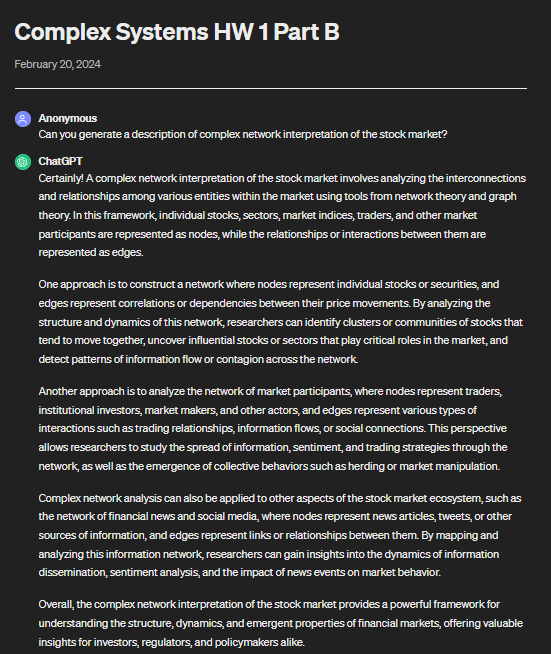
\includegraphics{prompt1.png}

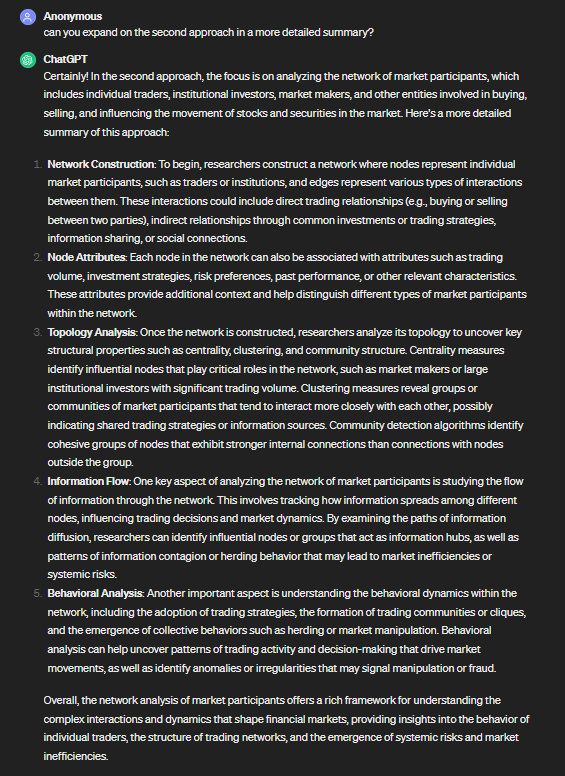
\includegraphics{prompt2.png}

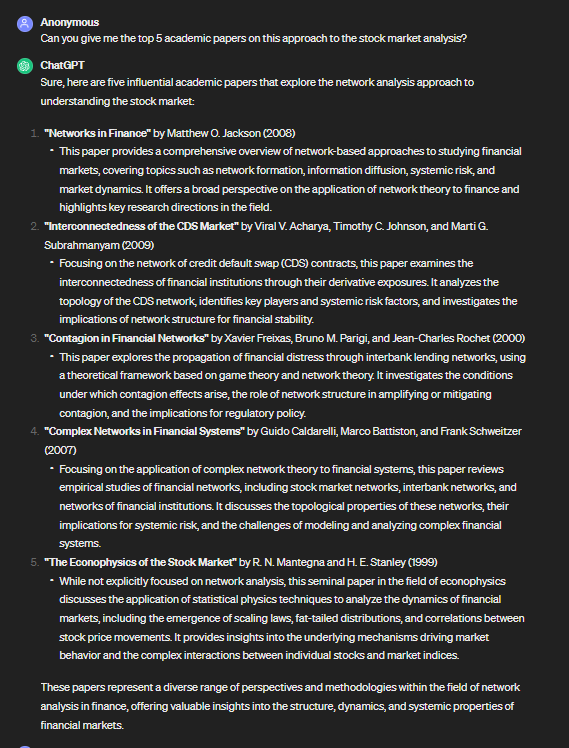
\includegraphics{prompt3.png}

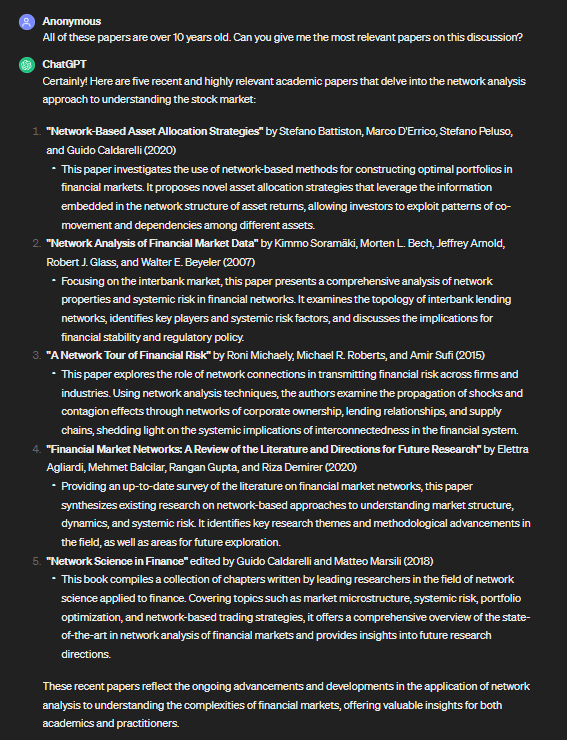
\includegraphics{prompt4.png}


\end{document}
